\section{
% SWE-agent
SWE-agent: Designing an ACI for Software Engineering
}
\label{sec:sweagent}
%\sandy{I am not sure what this section aims to do. It may be better focused if it solely discusses components of the ACI and you remove a lot of the introductory text about benchmarking, which you include later, and about the role of the ACI, which should be moved into Section 2.}
%\sandy{In light of this comment, consider deleting the following par.}
% SWE-agent uses an ACI that lets an LM act as a software engineering agent.
% To evaluate our system, we use SWE-bench, a benchmark for evaluating LMs on real-world software tasks collected from GitHub~\citep{jimenez2024swebench}.
% SWE-bench's issue resolution tasks reflect an important responsibility of software engineers, i.e., given a codebase and a natural language request (e.g. feature request, bug report), generate a codebase revision (a patch) that passes unit tests verifying that the issue has been remedied.
% Solving these tasks requires performing many software engineering sub-tasks, including bug localization, program repair, and writing tests to verify correctness.

%\sandy{Consider deleting the following sentence and saving the content of "A well-designed ACI should..." This discussion should begin Section 2 and be based on the needs assessment in Section 1.}
% SWE-agent overcomes these challenges by introducing powerful, tailored tools to provide agents with a simplified interface to the computer, the agent-computer interface (ACI).
% The ACI is responsible for managing interactions between the agent and computer, which includes providing shell commands, documentation, prompt directives, and managing the agent's memory.
% A well-designed ACI should help the LM agent understand the state of the repository given the previous changes, recover from mistakes, remove unnecessary context from prior observations, and suppress unusual or lengthy program outputs.


Here we describe how SWE-agent provides an ACI for LMs to act as software engineering agents, enabling them to effectively search, navigate, edit, and execute code commands.
The ACI comprises several principal components, including search/navigation, file viewer, file editor, and context management.
At each step, SWE-agent generates a thought and a command, then incorporates the feedback from the command's execution in the environment (ReAct;~\citet{yao2023react}).
Built atop the Linux shell, SWE-agent also allows access to common Linux commands and utilities when needed.

% SWE-agent provides an ACI for LMs to act as software engineering agents, helping them effectively search, navigate, edit, and execute code commands.
% Here we describe the principle components of SWE-agent for {\bf search / navigation}, {\bf file viewer}, {\bf file editor}, and {\bf context management}.
% At each step, SWE-agent generates a thought and a command, then incorporates the feedback from the command's execution in the environment (ReAct;~\citet{yao2023react}).
% Built atop the Linux shell, SWE-agent allows access to common Linux commands and utilities.

% It does this through the careful design of its principle components: {\bf search / navigation}, {\bf file viewer}, {\bf file editor}, and {\bf context management}.
% At each step, SWE-agent generates a thought and a command, then incorporates the feedback from the command's execution in the environment (ReAct;~\citet{yao2023react}).
% Built atop the Linux shell, SWE-agent allows access to common Linux commands and utilities.
% We describe the ACI components of SWE-agent below.
% \alex{Should we mention ReAct prompt/basic interaction loop?} \ofir{already mentioned in intro. ok to re-describe if you have space though.} \ofir{also note that i don't think we ever described the meaning of the 'thought' thing from ReACT in the paper. maybe would be good to spend a sentence on that somewhere.}

\textbf{Search and navigation.}
Navigating codebases requires finding the relevant file and content.
A common strategy to do this involves looking up terms that might be useful, e.g., files, functions, or class definitions mentioned in an issue. 
% Based on the principles of simple actions and informative feedback described in Section~\ref{sec:aci}, we implement search actions that only takes search terms as arguments with corresponding observations that are easy to interpret and act on.
We introduce the special commands \texttt{find\_file}, \texttt{search\_file}, and \texttt{search\_dir}, which output a summary of search results when searching for filenames and strings within files or directories.
Figure~\ref{fig.appx.swe_agent_components} shows examples of these search result formats. 
The \texttt{find\_file} command searches for filenames in the repository, while the \texttt{search\_file} and \texttt{search\_dir} locates strings in a file(s) of a subdirectory. Our interface encourages efficient searches by suppressing verbose results. The search commands return at most \num{50} results for each search query; if a search exceeds this number, we do not report the results and instead suggest that the agent write a more specific query.

\begin{figure}
  \centering
  \begin{subfigure}[t]{0.48\textwidth}
    \centering
    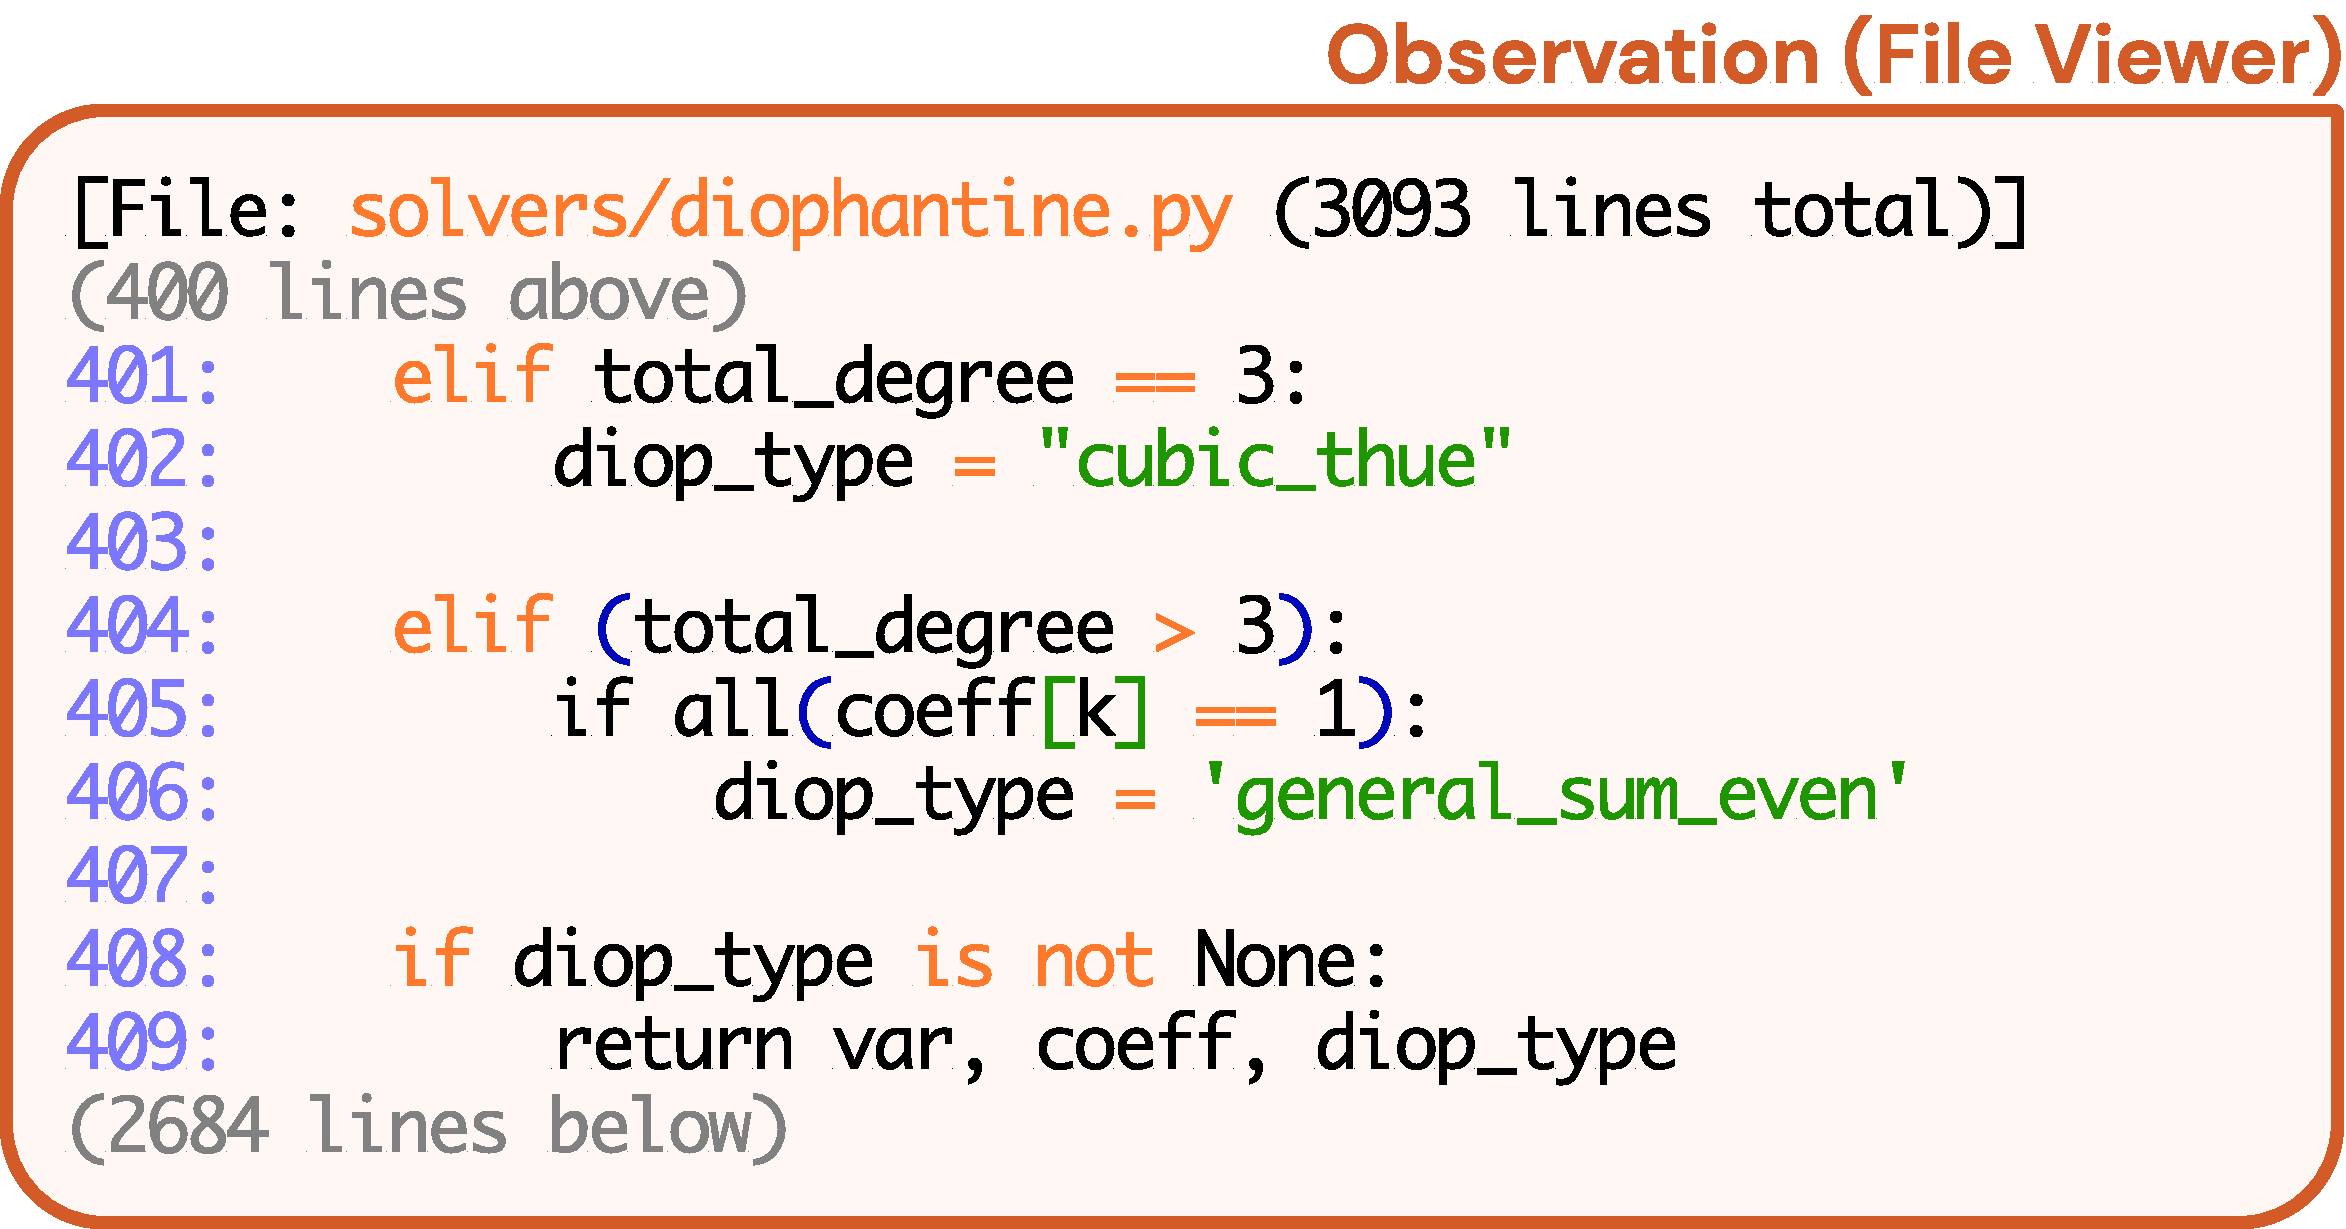
\includegraphics[width=\textwidth]{figures/file_viewer_example.pdf}
    \caption{Observation from the file viewer.}
    \label{fig:sub_viewer}
  \end{subfigure}
  \hfill
  \begin{subfigure}[t]{0.48\textwidth}
    \centering
    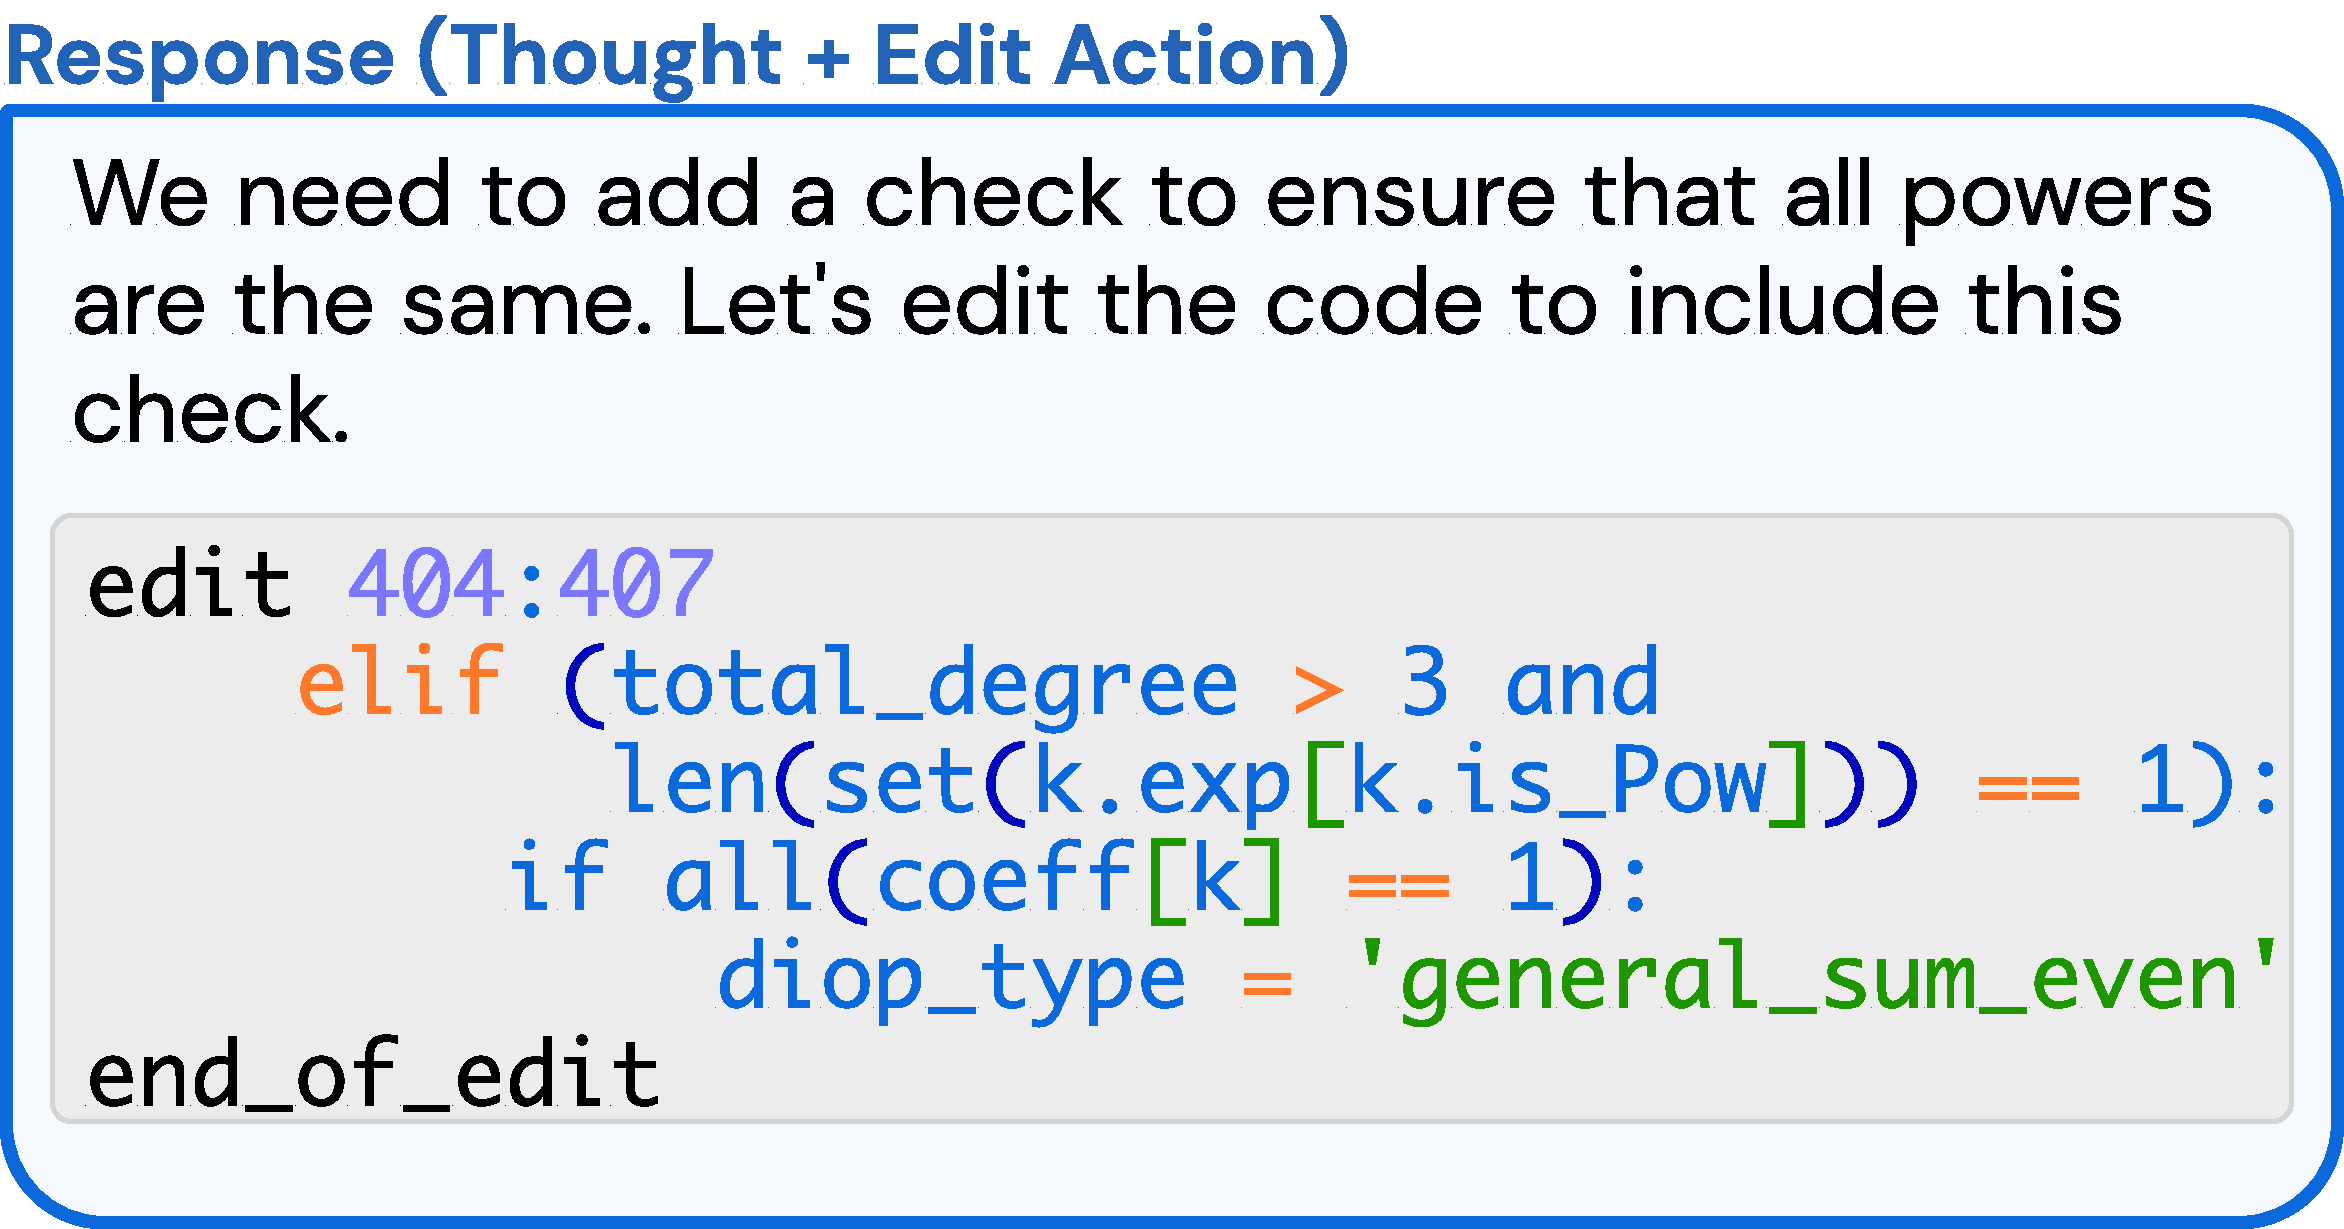
\includegraphics[width=\textwidth]{figures/file_editor_example.pdf}
    \caption{Action using the edit interface.}
    \label{fig:sub_editor}
  \end{subfigure}
  \caption{
  The file viewer and edit command are integrated.
  (a) The file viewer shows the agent the open file's content with line numbers. (b) The agent invokes the edit function to replace lines 404-407 in the open file.
  After the edit, the file viewer shows the agent the now updated version of the file.
  }
  \label{fig:viewer_and_editor}
\end{figure}

\textbf{File viewer.}
After finding a file they want to view, agents use the interactive file viewer by calling the command \texttt{open} on the relevant file path.
The file viewer presents a window of at most \num{100} lines of the file at a time.
The agent can move this window with the commands \texttt{scroll\_down} and \texttt{scroll\_up} or access a specific line with the \texttt{goto} command.
To facilitate in-file navigation and code localization, we display: the full path of the open file, the total number of lines in the file, the number of lines omitted before and after the current window, and the line number (prepended to each visible line). 
Figure~\ref{fig:sub_viewer} shows an example of this interface.

\textbf{File editor.}
We provide a few commands that let LMs create and edit files.
The \texttt{edit} command works in conjunction with the file viewer, allowing agents to replace a specific range of lines in the open file.
This command takes 3 required arguments: the start line, end line, and replacement text.
In a single step, agents can replace all lines between the start and end lines with the replacement text, as shown in Figure~\ref{fig:sub_editor}.
After edits are applied, the file viewer automatically displays the updated content, helping the agent observe the effects of its edit immediately without invoking additional commands. Figure~\ref{fig:sub_editor} shows an example agent response, including a file edit. 

Similar to how humans can use tools like syntax highlighting to help them notice format errors when editing files in an IDE, we integrate a code linter into the \texttt{edit} function to alert the agent of mistakes it may have introduced when editing a file.
Select errors from the linter are shown to the agent along with a snippet of the file contents before/after the error was introduced.
%\sandy{Below is a case where the 'who's doing what' is not clear because of passive voice. Do you mean, "The ACI (or is it SWE-agent?) discards invalid edits and asks the LM to try editing the file again."? }
Invalid edits are discarded, and the agent is asked to try editing the file again.

\textbf{Context management.}
The SWE-agent system uses informative prompts, error messages, and history processors to keep agent context concise and informative.
%\sandy{Re below, from whom do agents receive instructions. Can you clarify the following in terms of what the LM, the ACI, and the computer are doing since it's unclear to me who's doing what.}
Agents receive instructions, documentation, and demonstrations on the correct use of bash and ACI commands.
At each step, the system instructs them to generate both a \emph{thought} and an \emph{action}~\citep{yao2023react}.
Malformed generations trigger an error response, shown in Figure~\ref{fig.prompts.error}, asking the agent to try again, which is repeated until a valid generation is received.
Once received, all past error messages except the first are omitted. 

The agent's environment responses display computer output using the template shown in Figure~\ref{fig.prompts.next_step}; however, if no output is generated, a specific message (``Your command ran successfully and did not produce any output'') is included to enhance clarity. To further improve context relevance, observations preceding the last $5$ are each collapsed into a single line, shown in Figure~\ref{fig.prompts.collapsed_obs}.
By removing most content from prior observations, we maintain essential information about the plan and action history while reducing unnecessary context, which allows for more interaction cycles and avoids showing outdated file information. \S\ref{appx:interface} provides further implementation details.
